\chapter{Literature Review}
\section{Previous works}
The development of big astronomical surveys has greatly increased the importance of automatic data classification and processing. The separation of photometric catalogs into stars and galaxies must be automated because there is simply too much data for human specialists to manually classify \citep{Kim2016}. These large surveys are aimed at generating astronomical catalogues which then can be used for further studies of the objects. This makes accurate classification a crucial step.

There are 3 major categories of galaxies according to their morphologies as per Hubble galaxy classification scheme \citep{Hubble}. Any manual classification and analysis of large datasets requires a considerable amount of time and effort. The categorization of galaxies is difficult and imprecise due to the complicated nature of galaxies and the characteristics of the pictures \citep{Khalifa}. For scenarios with several categories, deep learning has shown notable results and significantly improved visual detection and identification.
The Convolutional Neural Network (CNN) is the most prevalent type of deep, feed-forward neural network (Don't understand this enough yet) and one of the most renowned deep learning algorithms \citep{Khalifa}. 

Neural networks consists of the model parameters and hyper parameters. Hyperparameter is a configuration that is external to the model and whose value cannot be determined from the data. With increasing complexity of CNN, the number of hyperparameter configurations to be determined increases \citep{Cui}.
One of the current practices to set hyperparameters is manual search, that is basically relying on human intuition and experience. The hyperparameters that work on one set of data are not guaranteed to work on another set of data \citep{Young}.
\pagebreak


HAVE TO COMPARE DIFFERENT METHODS USED IN DIFFERENT PAPERS.

SVM\citep{Zhang2012} vs kNN vs GAs to be compared. \citep{Philip} \citep{Wierzbiński}

\section{Genetic Algorithms (GAs)}
According to Darwin's rule of natural selection, organisms with phenotypes that are well matched to their immediate environment will eventually have a higher probability of reproducing and/or surviving than other, less suitable species \citep{DODSON1976243}. In the following generations, only those phenotypes prevails which are more suited to the environment. Mutation of genes can cause the organism to either have better characteristics or worse characteristics. But natural selection will eventually carry forward those mutations which are better.\par
Genetic Algorithm (GA) is a computational model which takes inspiration from Darwin's law of natural selection. The terminologies used to describe such types of algorithms are analogous to the biological ones. A population-based search technique called the Genetic Algorithm (GA) creates new populations by repeatedly using genetic operators or randomization functions \citep{Katoch2021}.GA effectively searches an encoded parameter space by using the objects from the population and the randomization technique \citep{Liu2019}.

A population is initialized using random variables (traits/characterstics), a set of variables is referred to as chromosomes. The main components of GA are chromosomal representation, crossover, fitness selection,  mutation, and fitness function computing. Until offsprings generated provide the ideal solution or the maximum number of iterations is achieved, the selection, crossover, and mutation procedures on the population are repeated. GA can be summaried in the form of a pseudo-code. \par



The fundamental theorem of GA is the Schema Theorem \citep{Liu2019}. ``According to Schema theorem, the original schema has to be replaced with modified schema. To maintain the diversity in population, the new schema keeps the initial population during the early stages of evolution. At the end of evolution, the appropriate schema will be produced to prevent any distortion of excellent genetic schema." \citep{Katoch2021} The most crucial element of genetic operators is the crossover operation. It is a recombination operator that joins pieces of the chromosomes of two parents to create offspring that have a portion of both parents' genetic makeup. \citep{Tang1996}. ``The offspring generation formed by the cross-interchange of the parental chromosomes is likely to discard or destroy the excellent genetic schemas possessed by the parental individual."\citep{Liu2019} \par

% url = {https://www.sciencedirect.com/science/article/pii/0025556476901279},

\subsection{Genetic Operators}
Genetic operators are the operators that are used during the optimisation process. See \autoref{fig:GAOperators} the general operators are encoding schemes, selection, crossover and mutation. 

\begin{figure}[H]
    \centering
    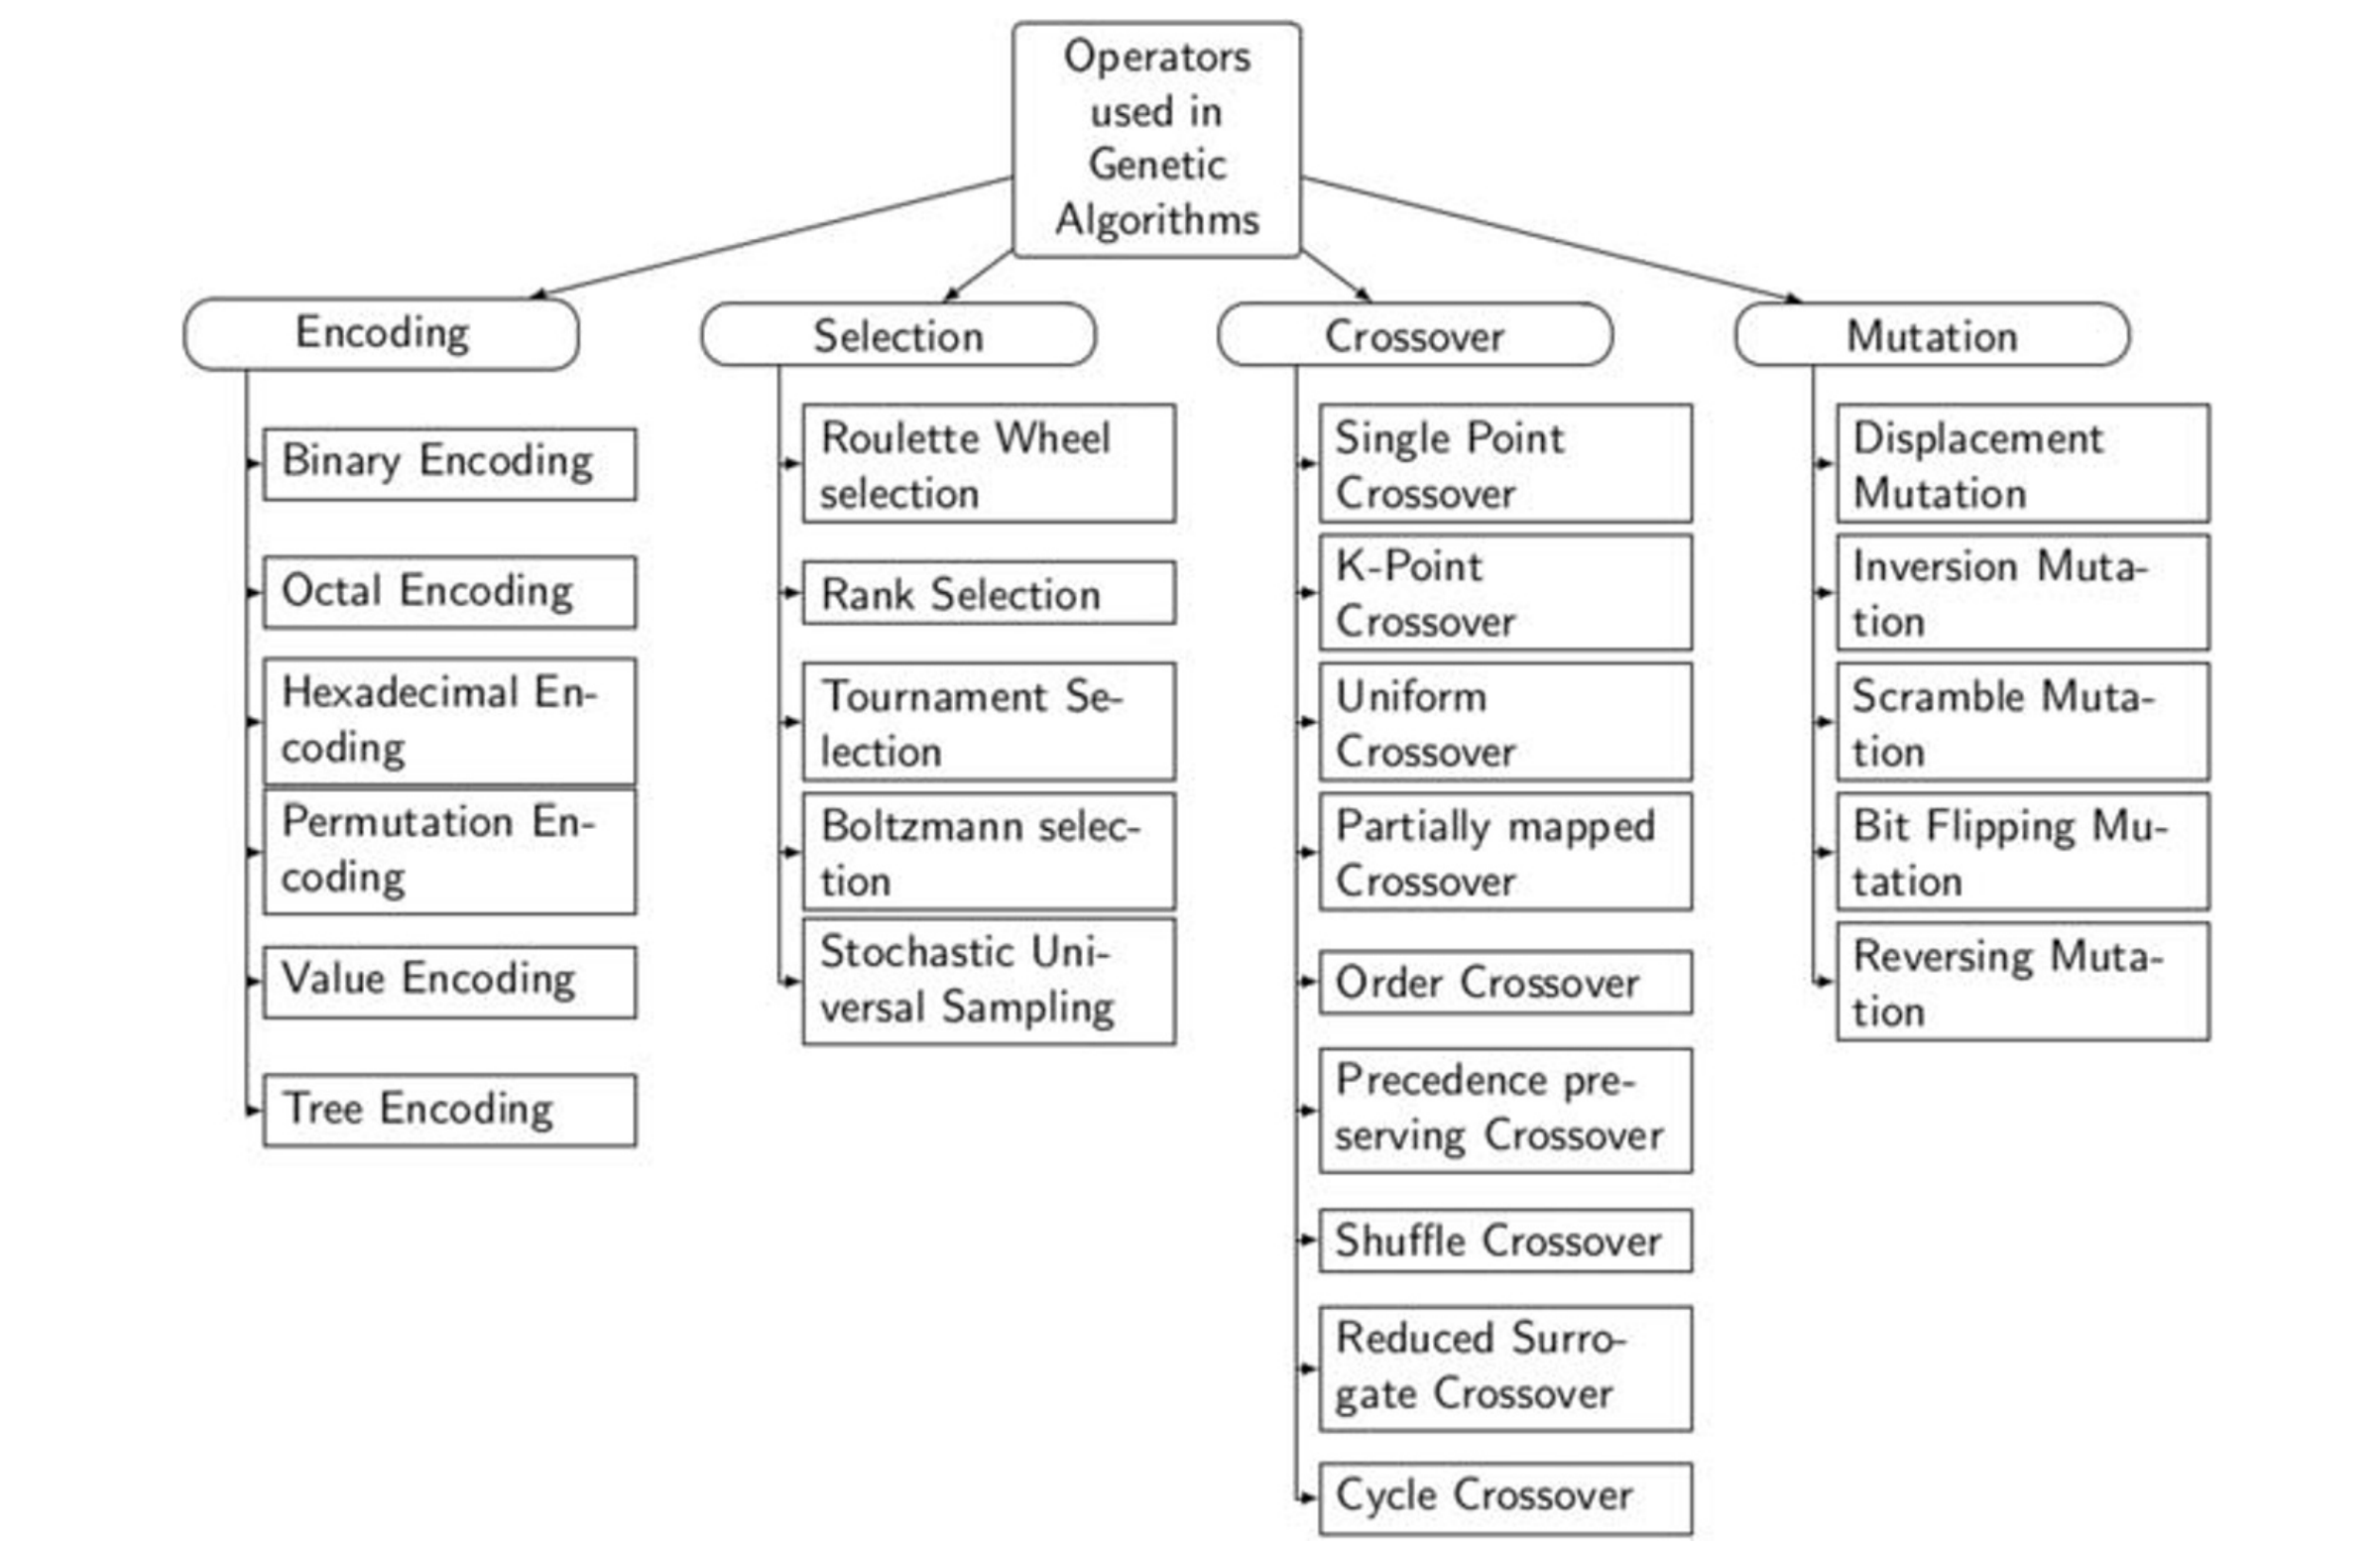
\includegraphics[scale=0.4]{images/GA_Operators.png}
    \caption{Operators used in Genetic Algorithms \citep{Katoch2021}}
    \label{fig:GAOperators}
\end{figure}

\subsubsection{Representation (Encoding Schemes)}
We encode the solution set of the problem to improve the algorithm's performance. This encoded object functions analogous to a chromosome. It is not the problem in itself, but rather a collection of attempted solutions to the problem. The chromosome can be represented / encoded as binary, octadecimal, or hexadecimal values, and these can then be subjected to crossover and mutation to provide a more likely set of solutions. Aside from numerical encoding, "permutation encoding" is generally preferred in ordering problems.

\subsubsection{Selection}
In genetic algorithms, selection is a key phase that determines whether  a particular string participates in reproduction. Boltzmann, rank, tournaments, roulette wheels, and  universal probabilistic sampling are examples of well-known selection techniques. The roulette wheel selection method maps all possible strings to the wheel and assigns each string a space on the wheel  based on the fit value. This wheel is then randomly rotated to select a specific solution involved in building the next generation \citep{Holland} \citep{Katoch2021}. \par
The modified version of roulettewheel selection is ranked selection. Instead of using fitness value, it uses rankings. Brindle introduced the tournament selection approach in 1983, in which the individuals are chosen in pairs from a stochastic roulette wheel based on their fitness scores. Following selection, those with a greater fitness value are added to the pool of the following generation. \citep{Holland}\par
The existing roulette wheel selection method is extended by stochastic universal sampling (SUS). It chooses an individual at regularly spaced intervals from a list of individuals from a generation, starting at a random position. All individuals have an equal chance of being chosen to take part in the following generation's crossover \citep{Katoch2021}.

\subsubsection{Crossover}
In order to create offspring, crossover operators combine the genetic information of two or more parents.

% The crossover formula is given as: 
% \begin{equation}
%     R = \frac{\left(G + 2 \sqrt{g}\right)}{3G}
% \end{equation}

% where $\mathbf{G}$ is the total number of evolutionary generations that have been set for this population in advance, and $\mathbf{g}$ is the amount the algorithm has ran for number of generations \citep{Liu2019}. \par
Many GA practitioners believe that the crossover operator is what really sets the GA apart from all other optimization algorithms. There are several crossover operation variants offered, with a single-point crossover being the most basic. Based on the selection methodology, the parents are randomly chosen. The regions of the two chromosomes beyond the crossover point are exchanged to create the offspring, where the crossover point is determined by a random process \citep{Tang1996}.\par
Similar to single-point crossover, multipoint crossover uses m crossover sites that are randomly selected without duplication. The crossover operator that is most often employed is partially matched crossover (PMX). This operator outperforms the majority of the other crossover operators in terms of performance \citep{Katoch2021}.

\subsubsection{Mutation}
An operator that modifies the chromosome is called mutation. The mutation can take place both on a global and local level. The procedure randomly changes the value of a string position occasionally (and typically with low probability $p$) \citep{Tang1996}. The three most well-known mutation operators are scramble mutation, simple inver-sion, and displacement.\par
The displacement mutation (DM) operator moves an individual solution's substring within itself. To ensure that both the final solution and a random displacement mutation are legitimate, the location is randomly selected from the substring that is being used for displacement. Exchange mutation and insertion mutation are two types of DM variations. A portion of a unique solution is either swapped with another portion or inserted in a different position in exchange mutation and insertion mutation operators, respectively. \citep{Jebari}\par
The SIM (simple inversion mutation operator) inversion operator flips the randomly chosen string and positions it in a random spot. Between any two given places in a single solution, the substring is reversed using the SIM \citep{Jebari}. The scramble mutation (SM) operator arranges the components of each individual solution in a random order and determines whether the freshly created solution's fitness value has increased or decreased \citep{Jebari}.